\documentclass[11pt]{article}
\usepackage[a4paper,margin=2.5cm]{geometry}
\usepackage[T1]{fontenc}
\usepackage[utf8]{inputenc}
\usepackage{lmodern,amsmath,amssymb,graphicx,booktabs,array}
\usepackage[numbers=false]{natbib}
\usepackage[hidelinks]{hyperref}
\bibliographystyle{plainnat}
\setcitestyle{authoryear,round,semicolon}
% Название — выбор автора; второй вариант: Represented but Not Reported: Probing Frozen Language Models as Embodied Readers
\title{Knowing More Than It Can Say: Frozen Language Models in Minimal Bodies}
\author{AUTHOR NAME (Latin script)\\ AFFILIATION\\ \texttt{EMAIL}\\ ORCID: 0000-0000-0000-0000}
\date{Preprint, October 2026}
\begin{document}
\maketitle
\begin{abstract}
Frozen pretrained language models are increasingly used as components of embodied agents, yet it is unclear what pretraining contributes in such settings and how much of what the model internally represents is available through its output. We study this in a minimal two-dimensional foraging environment where an agent's body events are presented to a frozen language model as a short sequence of discrete tokens, and compare each pretrained model against the same architecture with random weights and matched embedding norms. Across three model families (Pythia, Qwen2.5, OLMo-2; 1--1.5B parameters, with Pythia up to 6.9B for some analyses), we find that: (i) the advantage of pretraining comes from sequence-processing machinery rather than word meaning --- arbitrary event words work as well as or better than meaningful ones; (ii) a latent episode variable that is never stated explicitly in the context is linearly decodable from hidden states with AUC 0.93--0.99, but the model's own answer to a direct question recovers it only at AUC 0.61--0.64, and in Pythia, in-context examples from other episodes do not close this gap; (iii) the meaning of a word (food vs. harmful) is fully present at that word's position but reaches the final position, where an episode-level readout would use it, at most weakly (0.97--1.00 vs. 0.51--0.62); and (iv) when word meaning conflicts with in-context experience, a statistically reliable trace of the experience reaches the answer but is substantially weaker than the meaning effect (4--28\% of it) and leaves the answers essentially unchanged. All primary analyses were preregistered with timestamped commits, use exact permutation or bootstrap tests with Holm correction, and include controls for confounds that produced false positives during the project, such as survivorship-induced frequency cues. Taken together, the results suggest that frozen language models in this regime represent substantially more about their embodied situation than they can express, and that the bottleneck lies in routing and expression rather than in representation.
\end{abstract}

\section{Introduction}\label{sec:intro}

Language models are increasingly proposed as components of systems that monitor and control physical processes --- as planners for embodied agents \citep{ahn2022,huang2022}, as policies initialized from pretrained weights \citep{li2022,reid2022}, and, in industrial settings, as diagnostic layers that interpret sensor streams and explain anomalies to human operators \citep{dave2024,li2026,liu2025}. In safety-critical infrastructure such as power generation, the value of such a component depends less on how fluent its explanations are than on whether what it says reflects what it has actually registered. A diagnostic layer whose verbal report diverges from its internal state is a liability: operators act on the report, not on the state.

This question is not hypothetical for us. The author operates gas-engine power generation and develops KONTUR, an observation-only monitoring system for a generator fleet that includes a machine-learning diagnostic layer producing technician-facing explanations. In that system no automated decision touches the plant; every action is taken by an operator. Deciding whether a language model can be trusted in such a role --- and what must be read from it, its output or its internal state --- requires knowing how much of what a model represents about a physical situation actually reaches its output.

We study this question in a deliberately minimal setting, designed to separate mechanisms rather than to be realistic. A simulated agent in a two-dimensional foraging environment experiences discrete body events --- which kind of item it ate and whether its energy rose or fell --- and these events are presented to a frozen pretrained language model as a short token sequence. A latent variable of the episode, which item kind is currently food, is never stated in the context; it can only be inferred from the conjunction of events. This lets us ask three precise questions: what pretraining contributes to processing such event streams, whether the latent variable is represented in the model's hidden states, and whether the model can report it when asked directly.

Across three model families, we find a consistent dissociation between representation and report. The latent variable is linearly decodable from hidden states almost perfectly, while the model's own answer recovers it only weakly; the meaning of a word is fully present at that word's position but barely reaches the position where an episode-level readout would use it; and when word meaning conflicts with in-context experience, the experience leaves a measurable but small trace in the answer and essentially does not change it. Pretraining contributes sequence-processing machinery that works equally well on arbitrary symbols, rather than the meaning of the words. Probing studies on factual knowledge have reported related gaps between what models encode and what they express \citep{orgad2024,gekhman2025,burns2022,azaria2023}. Unlike prior studies of hidden factual knowledge, our target variable is not stored in pretrained parameters: it is constructed online from the agent's current experience.

Our contributions are:
\begin{enumerate}
\item a controlled setting in which a latent situation variable must be inferred from in-context body events, with a random-weight control of the same architecture for every comparison;
\item measurements of the gap between representation and report --- for a latent episode variable, for word meaning and for meaning against experience --- replicated across Pythia, Qwen2.5 and OLMo-2, which we interpret as a three-layer picture of representation, routing and expression;
\item a preregistered methodology with timestamped commits and a registry of all attempts, including a documented set of confounds that misled or would have misled our conclusions during the project --- survivorship-induced frequency cues, shortcuts through the agent's own closed-loop behavior, information loss in symbolic interfaces, and readout artifacts --- together with the controls that caught them.
\end{enumerate}

We make no claim that these findings transfer directly to deployed monitoring systems, which use larger models, richer inputs and often trained output channels. The practical implication we draw is narrower: in a role where a language model's output is taken as evidence about a physical system, the correspondence between its output and its internal state should be measured rather than assumed.


\section{Setup}

\subsection{Environment}

All analyses use a minimal two-dimensional foraging world, \emph{flip-2} . An episode lasts 100 steps  in the unit square, with two items of each of two kinds, A and B . In every episode one kind is food (+0.35 energy) and the other is poison ($-$0.20) . Which kind is food --- the \emph{episode sign} --- is drawn by a coin at the start, flips once at a random step between 30 and 69 , and is never observed directly. The body reports only events: which kind, if any, was eaten on this step, and whether energy went up, down, or stayed the same. Energy drifts down without food, so the body has its own time. For the analyses reported here, trajectories are generated by a \emph{blind} policy, a reflex that steers to the nearest item of either kind. The model therefore reads experience that it did not shape, and closed-loop shortcuts through behavior are excluded .

\subsection{Interfaces}

\textbf{Event words.} Each step is written as two tokens: the kind eaten (`` A'', `` B'', or `` none'') and the outcome (`` up'', `` down'', or `` same''). The window is preceded by a start token and covers the last 32 steps . The episode sign is not stated anywhere in the window. It can only be inferred by binding a kind to the outcomes that follow it. In an earlier interface, a fixed random projection of continuous sensor features into embedding space, pretrained models did not outperform random ones (Section 3.1). For the arbitrary-word control (Section 3.2), the six event words are replaced by unrelated single-token words (e.g. `` cat'', `` table'', `` stone'' / `` river'', `` chair'', `` door'') .

\textbf{Questions.} To read the model's \emph{answer}, a question is appended to the window (`` Food:'', `` Safe to eat:'', `` Good kind:''), and the answer is the logit difference between `` A'' and `` B'' at the last position .

\textbf{Kind words with meaning.} To test meaning (Section 3.4), the two kind symbols are replaced by words whose meaning is food (e.g. apple, bread) or harmful (e.g. mold, glass). These come from pools of 30 single-token words each, and words that name edibility directly are excluded .

\textbf{Synthetic windows.} To separate meaning from experience without any frequency cue (Section 3.5), we construct windows of short sentences (``I ate w. Energy went up.'' / ``\ldots{} went down.'' / ``Nothing happened.'').
\begin{itemize}
\item Each window contains n ∈ \{2, 4, 6\} events, with exactly n/2 per kind. The kinds of the first and last events, and the reference kind used for scoring, are balanced within every cell .
\item A frequency reference, a last-mentioned reference and a first-mentioned reference all score exactly 0.5 on these windows. A Bayesian reader of the kind--outcome binding scores 1.0 .
\item The control keeps words, positions and order, and permutes outcomes across events so that the binding is uninformative .
\item Ten sets of 648 windows are used .
\end{itemize}

\subsection{Models and controls}

\begin{itemize}
\item \textbf{Models:} Pythia 160M--6.9B, Qwen2.5-1.5B and OLMo-2-1B, all frozen and run in fp32 with TF32 disabled .
\item \textbf{Random-weight control.} Every pretrained model is compared with the same architecture with random weights; its input embeddings are rescaled to the mean row norm of the pretrained embeddings . The random network is reseeded for every set, except in the meaning probe (Section 3.4), which uses one random network per model .
\item \textbf{Tokenizer transfer.} For the cross-family replication, every protocol was transferred without other changes :
\begin{itemize}
\item the start token is each model's end-of-document token, ``<|endoftext|>''. It is the BOS token in Pythia and OLMo-2; Qwen2.5 has no BOS by default ;
\item every word is a single token with a leading space in all three tokenizers, so no substitutions were needed ;
\item all inputs were verified by decoding;
\item Pythia-1B run through the transferred code reproduced the original numbers (e.g. 0.983 / 0.526 / 1.000 for the meaning probe) .
\end{itemize}
\end{itemize}

\subsection{Measures}

\textbf{Probes.} Probes are L2-regularized logistic regressions on the final-layer hidden state. Features are standardized on the training part of each fold, and the regularization strength is chosen by inner validation . Folds are grouped by episode when the probe is tested on new episodes with the same symbols (Sections 3.1--3.3). When the probe must generalize to new words, folds are grouped by word, so test words are never seen in training (Section 3.4) . The sign probe reports balanced accuracy ; the other probes report AUC.

\textbf{Answers.} Answers are logit differences between the two answer tokens after a question, scored by AUC against the true sign , or as mean logit shifts (Section 3.5) . Reading logits rather than sampled text follows the argument that prompted judgments can understate what a model encodes \citep{hu2023}.

\subsection{Statistics and preregistration}

\begin{itemize}
\item \textbf{Main test.} Exact paired sign-flip permutation tests over 10 sets (1,024 permutations), one-sided where the direction was preregistered  and two-sided in the earliest analyses .
\item \textbf{Meaning probe.} It used a one-sided bootstrap (10,000 resamples) .
\item \textbf{Intervals.} Where a probe generalizes to new words, intervals are cluster bootstraps over words, not over episodes . Other intervals are 95\% t-intervals over sets.
\item \textbf{Multiplicity.} Holm correction within each preregistered family.
\item \textbf{Preregistration.} Every primary analysis was preregistered in a commit made before any data were computed, with all outcomes and their interpretation written down in advance. Every attempt, including abandoned environment variants, is listed in a registry . Analyses added after seeing data are labeled post hoc.
\end{itemize}

\section{Results}

\subsection{The interface decides whether pretraining helps}
\begin{figure}[t]\centering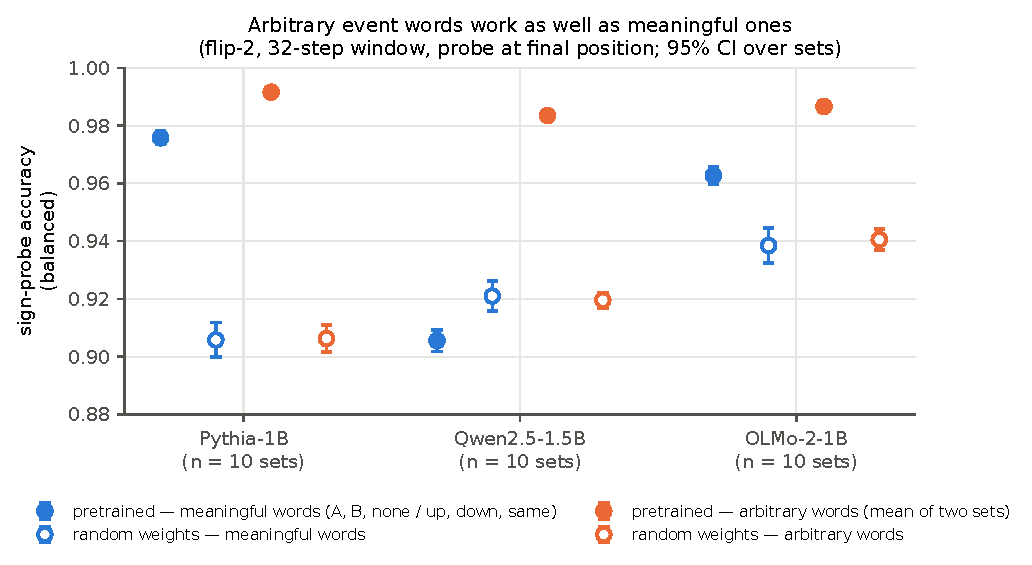
\includegraphics[width=\linewidth]{figures/F2_words_vs_random.pdf}
\caption{\textbf{Meaningful vs. arbitrary event words..} Balanced accuracy of a linear probe for the episode sign at the final window position, with meaningful event words (A, B, none / up, down, same; blue) or arbitrary single-token words (mean of two word sets; orange); filled: pretrained, hollow: random weights. 10 sets $\times$ 200 episodes per model; mean and 95\% t-interval over sets. Data: A28 (protocols of A3 and A4).}\label{fig:F2}\end{figure}

\textbf{Continuous projector.} Pretrained Pythia was no better than random weights when body states entered through the continuous projector: at 160M it was significantly worse ($-$0.053, Holm p = 0.012) .

\textbf{Start token and event words.} Adding a start token removed most of the gap: at 160M the pretrained--random difference went from $-$0.054 to $-$0.008, an improvement of +0.047 (Holm p = 0.004) . Writing events as words gave pretrained models their first advantage: relative to the projector interface, the pretrained--random gap improved by +0.191 (Holm p = 0.004), giving sign-probe balanced accuracy 0.950 vs. 0.813 at 160M , and, descriptively, 0.951 vs. 0.856 at 410M .

\textbf{Replication.} The advantage replicates on OLMo-2-1B (0.963 vs. 0.938, Holm p = 0.006)  and, descriptively, on Pythia-1B (0.976 vs. 0.906) . It does \textbf{not} replicate on Qwen2.5-1.5B with these event words: 0.906 vs. 0.921, with the pretrained model lower in 9 of 10 sets . With arbitrary event words, pretrained Qwen2.5 is again clearly ahead (0.983 vs. 0.920)  (Fig. F2). We did not investigate why the letter-like symbols disadvantage Qwen2.5. The claim that event words let pretraining help therefore holds with a caveat about model family and symbol set.

\subsection{Machinery, not meaning}

\textbf{Pythia-160M.} If the advantage came from the meaning of the event words, unrelated words should remove it. They do not. At 160M, arbitrary words were \emph{better} than meaningful ones by 0.016 (Holm p = 0.004), and pretrained models on arbitrary words beat random weights by 0.156 (Holm p = 0.004) . Replacing the six event embeddings of the pretrained model with random vectors of the same norm still gave, descriptively, 0.984 . An apparent preference for one arbitrary word set was later traced to token luck, so we state the result as ``not worse'' rather than ``better'' .

\textbf{Replication.} Across the three families, arbitrary words are non-inferior to meaningful ones and above random weights (Holm p = 0.006 in Qwen2.5 and OLMo-2 for the preregistered test requiring both; Pythia-1B descriptively) . The differences against meaningful words are +0.016 for Pythia-1B, +0.078 for Qwen2.5 and +0.024 for OLMo-2  (Fig. F2).

What pretraining contributes here is sequence-processing machinery over discrete symbols, not the meaning of the symbols. This parallels findings that language-model initialization helps decision making whether or not inputs are natural language \citep{li2022}, and that random transformers already have some algorithmic capabilities \citep{zhong2024}.

\subsection{Represented but not reported}
\begin{figure}[t]\centering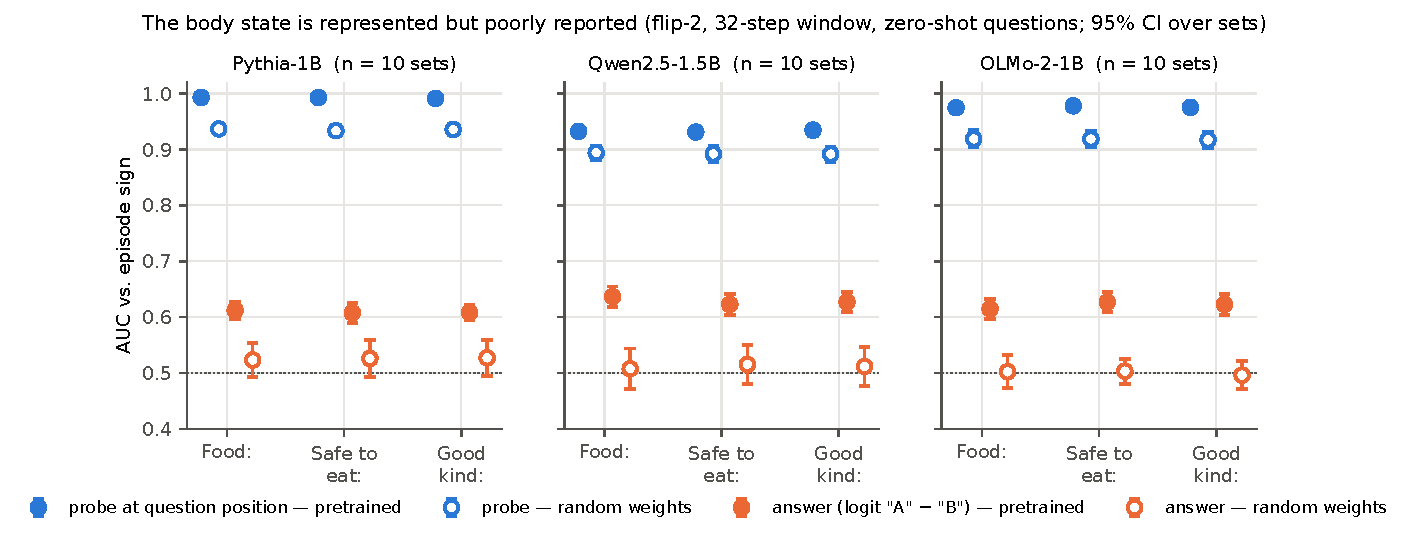
\includegraphics[width=\linewidth]{figures/F1_probe_vs_answer.pdf}
\caption{\textbf{Probe vs. answer for the latent episode sign..} AUC against the episode sign of a linear probe at the question position (blue) and of the model's answer, the logit difference `` A'' $-$ `` B'' (orange), for three zero-shot questions. Filled markers: pretrained; hollow: the same architecture with random weights and matched embedding norms. flip-2, 32-step event-word window; 10 sets $\times$ 100 episodes per model; mean and 95\% t-interval over sets. Data: A28 (protocol of A22).}\label{fig:F1}\end{figure}

\textbf{Representation.} The episode sign is never stated in the window, yet a linear probe at the question position decodes it with AUC 0.993, 0.932 and 0.975 (Pythia-1B, Qwen2.5, OLMo-2; first question) .

\textbf{Answer.} Asked directly, the same models answer far worse: AUC 0.607--0.612, 0.623--0.637 and 0.615--0.627 across the three questions . This repeats the original Pythia result (zero-shot AUC 0.61 against a probe at 0.98--0.99) .

\textbf{Preregistered criterion.} The answer's excess over chance is at most half of the probe's, (AUC\_answer $-$ 0.5) $\le$ 0.5 $\cdot$ (AUC\_probe $-$ 0.5). It holds for all three questions in all three families  (Fig. F1). The probe is trained on the hidden state at the same position from which the answer is read; it is thus a trained linear bridge from that state. The gap between the probe and the answer therefore points to the mapping from this state to the answer tokens, rather than to an absence of the information at this position.

\textbf{Two observations qualify this picture.}
\begin{itemize}
\item Random-weight networks also support high probes (0.892--0.937), while their answers stay at chance (0.50--0.53) . Descriptively, pretraining adds more to the answer channel (+0.09 to +0.13 AUC) than to the probe (+0.04 to +0.06) . We did not test this difference.
\item In Pythia only, in-context examples did not close the gap. Examples from the same episode were simply copied: few-shot AUC 0.974 matched a ``repeat the last example's answer'' control at 0.975 . Examples from other episodes gave chance (AUC 0.505 at 160M, 0.469 at 1B), not above random weights or the copy control (Holm p $\ge$ 0.6) . A23 was run on Pythia only.
\end{itemize}

The pattern --- internal states that encode more than the model's output reveals --- has been reported for factual knowledge and truthfulness \citep{orgad2024,gekhman2025,azaria2023}; here it concerns a variable that exists only in the agent's recent bodily experience.

\subsection{Meaning stays local}
\begin{figure}[t]\centering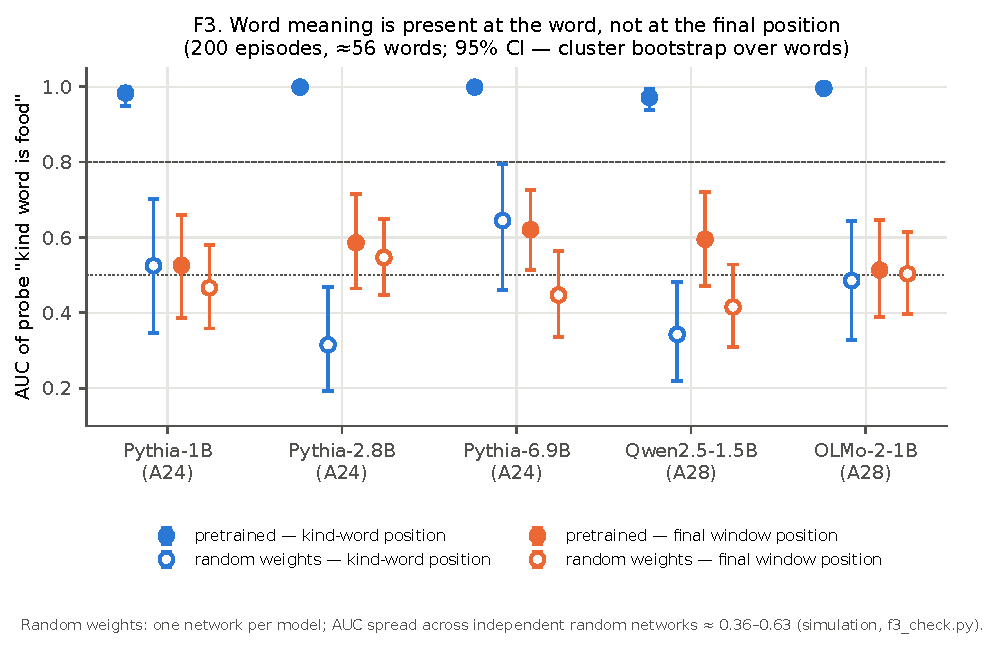
\includegraphics[width=\linewidth]{figures/F3_meaning_by_position.pdf}
\caption{\textbf{Word meaning by position..} AUC of a linear probe for ``the kind word denotes food'', tested on words never seen in training, read at the kind word's own position (blue) and at the final window position (orange); filled: pretrained, hollow: random weights. Pythia 1B / 2.8B / 6.9B from A24 and Qwen2.5-1.5B / OLMo-2-1B from A28 were computed on different RTX 5090 instances; the comparison across these groups is descriptive. 200 episodes, $\approx$56 distinct test words; 95\% cluster-bootstrap intervals over words. Random weights: one network per model; across independent random networks the AUC spreads over $\approx$0.36--0.63 (simulation). Dashed line: preregistered threshold 0.8.}\label{fig:F3}\end{figure}

\textbf{Meaning in language.} The models know which words denote food. A probe on the word's hidden state in a neutral sentence (``The apple.''), tested on held-out words, separates food from harmful words with AUC 1.000, 1.000 and 0.999 for Pythia 1B, 2.8B and 6.9B , and 1.000 for Qwen2.5 and OLMo-2 . Direct words (edible vs. poison) serve as a positive control for the method (1.000 / 0.967 / 0.967; 0.900; 0.967) .

\textbf{Meaning in the event window.} When the same words appear as kind symbols, the probe --- tested on words never seen in training --- reads their meaning at the kind word's own position: 0.983--0.999 for Pythia , 0.972 for Qwen2.5 and 0.996 for OLMo-2 . At the final position, where an episode-level readout would look, it reaches at most 0.53--0.62: 0.526 / 0.586 / 0.620 for Pythia 1B / 2.8B / 6.9B , 0.595 for Qwen2.5 and 0.514 for OLMo-2  (Fig. F3).

\textbf{Intervals.} Because the probe generalizes to new words, intervals are cluster bootstraps over the $\sim$56 test words. For Pythia-6.9B at the final position, this gives 0.620 [0.51, 0.73] against 0.447 [0.33, 0.56] for random weights . We therefore do not claim that 6.9B carries more meaning to the final position than a random network. We claim only that no model reaches the preregistered threshold of 0.8 .

\textbf{Random-weight values below 0.5.} These (e.g. 0.315 for Pythia-2.8B) are not an artifact of the word-grouped split. A simulation of the same procedure on random word vectors gives a mean of 0.495, with independent random networks spread over 0.36--0.63 .

The meaning of a word is thus present where the word is, but is not routed to the position that summarizes the episode. This is consistent with work on how models bind attributes to entities in context \citep{feng2023}.

\subsection{Meaning against experience: a weak trace that does not change answers}
\begin{figure}[t]\centering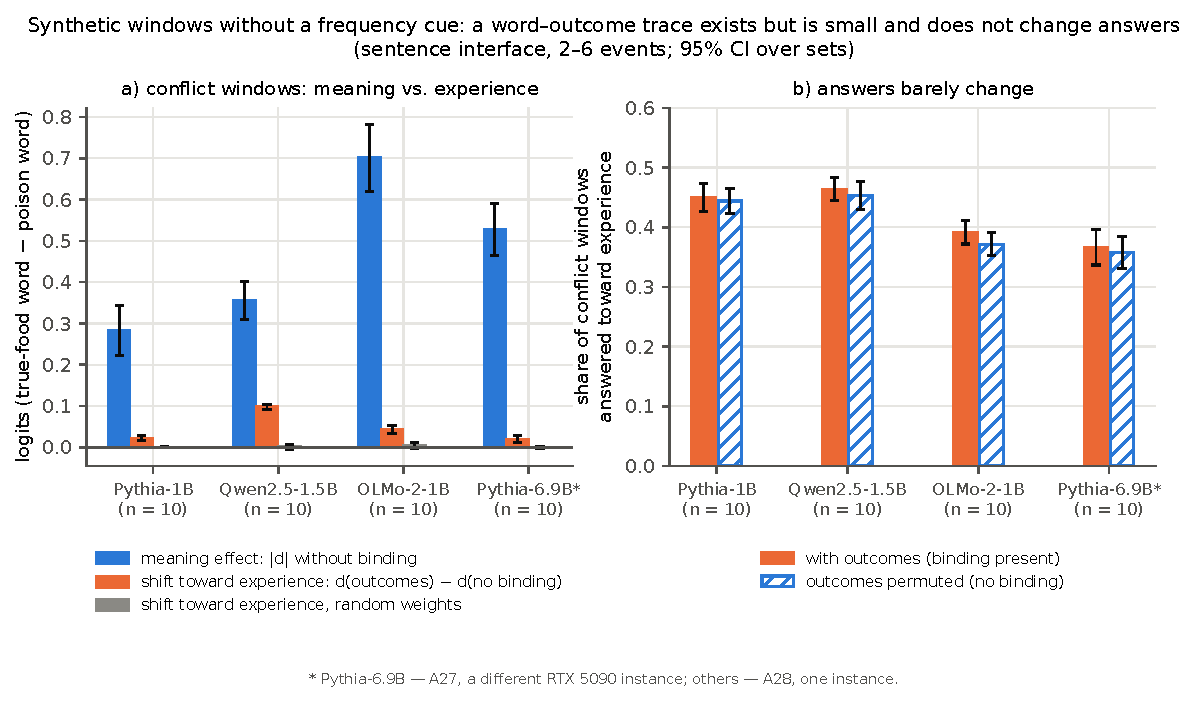
\includegraphics[width=\linewidth]{figures/F4_synthetic_binding.pdf}
\caption{\textbf{Meaning against experience in synthetic windows..} (a) On conflict windows (kind words whose meaning contradicts the outcomes): the meaning effect, |d| on the same windows with outcomes permuted (blue); the shift toward experience, d(outcomes) $-$ d(permuted) (orange); the same shift for random weights (grey); d is the logit difference between the true-food word and the poison word. (b) Share of conflict windows answered toward experience, with outcomes (orange) and with outcomes permuted (hatched). Sentence interface, 2--6 events per window, 10 sets $\times$ 648 windows; mean and 95\% t-interval over sets. Pythia-1B, Qwen2.5-1.5B, OLMo-2-1B: A28 (one instance); Pythia-6.9B: A27 (a different instance).}\label{fig:F4}\end{figure}

\textbf{Why synthetic windows (post hoc, Pythia).} A first test used simulated bodies (Pythia 1B--6.9B) .
\begin{itemize}
\item Kind words were truthful, lying (a food word naming the poisonous kind) or neutral.
\item The preregistered shift toward experience was formally positive in all six cells. But it persisted when kind and outcome slots were shuffled .
\item Post hoc, we traced it to survivorship: queries came only from living bodies, so the food kind had been eaten more often (frequency reference 0.62 instead of the assumed 0.5) . The answer followed the more frequently mentioned word, at +1.1 to +1.9 logits per mention .
\item With equal mentions, the shift vanished in 5 of 6 cells .
\end{itemize}

This frequency channel is what the synthetic windows remove.

\textbf{Synthetic windows.} We compare windows where the kind words lie, against the same windows with outcomes permuted (Fig. F4).
\begin{itemize}
\item In Pythia-6.9B, experience moves the answer toward the true food by +0.020 logits relative to permuted outcomes, more than it does in random weights (Holm p = 0.002 for the preregistered test requiring both comparisons). This is small against a meaning effect of $-$0.51 .
\item The shift replicates in Qwen2.5 and OLMo-2 (Holm p = 0.006; Pythia-1B descriptively), with random weights near zero : +0.022 (Pythia-1B), +0.098 (Qwen2.5), +0.044 (OLMo-2) logits.
\item Relative to the meaning effect, the shift is 3.8\% (Pythia-6.9B), 7.7\% (Pythia-1B), 6.3\% (OLMo-2) and 27.6\% (Qwen2.5) .
\item Descriptively, it does not grow from 1B to 6.9B in Pythia .
\item The answers themselves barely change. The share of conflict windows answered toward experience is 0.450 vs. 0.444 with and without the binding for Pythia-1B, 0.464 vs. 0.453 for Qwen2.5, 0.392 vs. 0.372 for OLMo-2 , and 0.36 vs. 0.36 for Pythia-6.9B .
\item The preregistered companion test --- that experience alone, with neutral kind words, is answered above random weights --- was not met: AUC 0.509 exceeded the permuted control (p = 0.001) but not random weights (0.489 $\pm$ 0.034, p = 0.105) .
\end{itemize}

A hint from the first test (Pythia-6.9B with sentences, +0.43 logits under equal mentions) did not survive the clean construction (+0.02) .

We conclude that the binding of a word to its outcome in context leaves a statistically reliable but small trace in the answer, and that when meaning and experience conflict, meaning decides.


\section{Pitfalls and controls}



Several results during the project looked like findings and were not. For each we give what happened, the false result it produced, and the control that caught it.

\textbf{Readout artifact in the original interface.} In the first interface, body states entered through a continuous projector, and the readout used the raw final hidden state. With that readout the pretrained Pythia lagged its random-weight twin, suggesting that pretraining hurts. Its hidden states were nearly collinear (cosine 0.986 between states) , consistent with a few very large activations dominating the representation \citep{sun2024}. With a fixed standardization of hidden states the difference disappeared: fitness (fraction of the episode survived plus half the final energy) 1.455 vs. 1.453 (3 seeds) and 1.453 vs. 1.457 in a ten-seed repeat (p = 0.20) . Standardized readouts have been the default since.

\textbf{Shortcuts through closed-loop behavior.} When a readout learns while the agent acts, the agent's own behavior becomes part of its input. In one series, a random-weight model appeared to read the episode sign better than the pretrained one, and a raw event window solved the task without a memory model . Out-of-loop evaluation on trajectories of a blind policy removed both effects.
\begin{itemize}
\item The raw window fell from 0.759 to 0.570: it had used a ``lost, so switch'' rule, not a memory of the sign .
\item The random-weight head fell from 0.670 to 0.513 .
\end{itemize}

All analyses in this paper use trajectories the model did not shape.

\textbf{A frequency cue created by survivorship.} In the first test of meaning against experience, queries came only from living bodies . Bodies that ate more poison were more often dead, so among the living the food kind had been eaten more often. A frequency reference that the preregistration assumed would score 0.5 by construction scored 0.62 . The preregistered shift toward experience was formally positive in all six cells but persisted when kind and outcome slots were shuffled. Post hoc, the answer followed the more frequently mentioned word, at +1.1 to +1.9 logits per mention; with equal mentions the shift vanished in 5 of 6 cells . We now check every ``0.5 by construction'' reference on the actual inputs before preregistering. The synthetic windows of Section 3.5 pass this check exactly .

\textbf{Information lost by a symbolic interface.} In a separate line of the project, input was quantized into event symbols. Before running any language model we computed what a simple rule could extract from them: 0.62, against 0.985 from the continuous sensors . The model then scored 0.48--0.52 . We recorded this null result with that caveat, not as a statement about language models.

\textbf{A condition against random weights that silently required a sign.} In the final meaning-versus-experience test, the preregistered condition required the pretrained answer on conflict windows to exceed that of random weights. By symmetry, random weights answer near zero there, so the condition demanded that experience \emph{outweigh} meaning, not merely shift the answer. We noticed this before computing any data. In a separate commit, the condition was replaced by a comparison of shifts relative to permuted outcomes; the original condition is reported descriptively .

\textbf{Intervals over observations instead of units of generalization.} The meaning probe of Section 3.4 is tested on unseen words, but its intervals and test resampled episodes . With about 56 distinct test words, this understates uncertainty: in a simulation of the same procedure, independent random networks spread over AUC 0.36--0.63 . Cluster bootstraps over words widened the intervals roughly 1.5--2$\times$. A preregistered claim that Pythia-6.9B carries more meaning to the final position than random weights can no longer be supported; the threshold verdict (below 0.8 for every model) is unchanged . Where a probe generalizes to new units, intervals and tests are now computed over those units.


\section{Discussion}

\textbf{A three-layer interpretation.} We read the results as pointing to three layers with very different capacities, while noting that this is an interpretation of the measurements rather than a measured mechanism. \emph{Representation} is rich: the episode sign is linearly decodable almost perfectly, and so is the meaning of a word. \emph{Routing} is limited: word meaning is present at the word's own position but barely reaches the position that summarizes the episode. \emph{Expression} is narrow: the answer channel recovers the latent sign only weakly, and when word meaning conflicts with in-context experience, the answer follows the word. On this reading, the bottleneck of a frozen model reading an embodied situation lies not in what it registers but in what reaches its output. We use representation, routing and expression as operational descriptions of the measurements --- linear decodability from a specified hidden state, the change in decodability between positions, and the effect on the model's answer distribution --- not as claims about separately localized mechanisms.

High probe accuracy alone does not show that a model uses the information \citep{hewitt2019,belinkov2021,elazar2020}, and our random-weight controls make this point concrete: random networks also support probes at 0.89--0.94 while answering at chance. Descriptively, what distinguishes pretrained models in our data is mainly the answer channel. We therefore treat the answer as the measure of observable use at the tested output channel, and the probe as an upper bound on what could be used --- in line with the observation that prompted judgments can understate what a model encodes \citep{hu2023}, and with reports that models encode more about facts than they express \citep{orgad2024,gekhman2025}.

\textbf{Why expression might lag.} One account, consistent with the data but not tested here, is that the answer channel is shaped by the statistics of pretraining text: it maps contexts to words through associations learned before the episode began. Word meaning is such an association, and it dominated the answers in every model we tested (Section 3.5); in Pythia, a post hoc analysis suggests that mention frequency acted the same way (Section 3.5). The episode sign is not such an association: it is a binding of a kind to its outcomes that exists only in the current context. Work on entity tracking \citep{kim2023} finds that models pretrained only on text track the state of entities poorly, while work on binding mechanisms \citep{feng2023} shows that sufficiently large models represent in-context bindings through specific internal mechanisms; our results add that a bound variable can be well represented and still fail to reach the output.

\textbf{Implications for monitoring critical systems.} The setting is minimal, and we do not claim direct transfer to deployed systems. Three practical implications nonetheless follow for any role in which a language model's output is taken as evidence about a physical process. First, the correspondence between output and internal state should be measured, not assumed: a fluent explanation may express less than the model has registered, or something other than it. Second, where ground truth is available, reading internal states with calibrated probes may be more faithful than reading the model's answer --- a suggestion we have not tested in a monitoring setting. Third, names carry priors: in our data the meaning of a word outweighed in-context evidence about the thing it named. In a monitoring setting, labels of components, alarms or states could likewise pull an answer toward what the label suggests rather than what the evidence shows --- a failure mode worth testing explicitly before a model's explanations are put in front of operators.

\textbf{Methodological lessons.} Several early results were misleading, and each was caught by a specific control: two false positives (shortcuts through the agent's own closed-loop behavior, and a frequency cue created by survivorship), one false negative (a readout artifact consistent with massive activations \citep{sun2024}), one null result that reflected information lost by a symbolic interface, and a condition against random weights that silently required a sign, caught before any data were computed. We list these not as contributions in themselves but as risks that apply to any evaluation of language models embedded in agents, where the data a model sees are shaped by the agent that produces them.

\textbf{Limitations.} Models are frozen and small: replication covers 1--1.5B parameters, and Pythia extends to 6.9B for some analyses. We did not study instruction-tuned models, whose answer channel is trained to report and may behave differently --- the most important open question for the practical implications above. The environment is a toy designed to separate mechanisms, not to resemble a real process. Probes are linear; high linear decodability indicates accessible information, but low decodability does not establish its absence; answers are read as a logit difference between two tokens rather than as free text. The cross-episode in-context test was run on Pythia only. Code was implemented and run with an AI coding assistant under the author's direction; all preregistrations, code and results are released.

\textbf{Future work.} Three directions follow directly: instruction-tuned and larger models; the minimal trainable bridge from internal state to answer --- how much plasticity a frozen model needs to report what it represents; and the same protocol on real sensor streams from an operating plant.


\section*{Disclosure}
Code implementation and experiment execution were performed with an AI coding assistant (Claude Code) under the author's direction; hypotheses, preregistrations, decisions to stop or continue each line, and interpretation are the author's. All code, preregistration commits, and results are released.

\bibliography{refs}

\appendix
\section{Replication and tokenizer transfer}



\textbf{Models.} Qwen2.5-1.5B (\texttt{Qwen/Qwen2.5-1.5B}) and OLMo-2-1B (\texttt{allenai/OLMo-2-0425-1B}), both without access restrictions. Pythia-1B was run through the same transferred code on the same machine as a reference; it was not part of the replication family. For every model, the random-weight control uses the same architecture, a network reseeded per set (one network, seed 1, for the meaning probe) and input embeddings rescaled to the pretrained mean row norm. All runs use fp32 with TF32 disabled.

\textbf{Start token.}
\begin{itemize}
\item Each model's end-of-document token, \texttt{<|endoftext|>}, is used as the start token: 0 in Pythia, 100257 in OLMo-2 and 151643 in Qwen2.5.
\item In Pythia and OLMo-2 this is the BOS token; Qwen2.5 has no BOS by default.
\end{itemize}

\textbf{Single-token words.}
\begin{itemize}
\item Every word used by the protocols is a single token with a leading space in all three tokenizers. This covers the event symbols, both arbitrary word sets and all meaning pools (30 food, 30 harmful, 30 neutral and 11 direct words). No substitutions were needed.
\item Token ids are taken from each tokenizer: for the event symbols A, B, none / up, down, same they are 362, 425, 6857 / 705, 1495, 1852 in Qwen2.5 and 362, 426, 7000 / 709, 1523, 1890 in OLMo-2.
\item In Pythia they are 329, 378, 5293 / 598, 1066, 1072, exactly the constants of the original scripts.
\end{itemize}

\textbf{Verification.}
\begin{itemize}
\item All inputs of all five protocols were decoded and inspected for the three tokenizers.
\item Hidden states are read as \texttt{base\_model(...).last\_hidden\_state} (after the final normalization). On a model outside the family this matched the last element of \texttt{hidden\_states} exactly, and logits matched hidden state $\times$ output embedding exactly.
\item Pythia-1B through the transferred code reproduced the original results:
\end{itemize}

\begin{center}\small\begin{tabular}{p{0.31\linewidth} p{0.31\linewidth} p{0.31\linewidth}}\hline
\textbf{Protocol} & \textbf{Transferred code} & \textbf{Original} \\ \hline
Meaning probe: kind position / final position / direct words & 0.983 / 0.526 / 1.000 & 0.983 / 0.526 / 1.000 \\
Synthetic windows: d on conflict windows, with / without binding & $-$0.262 / $-$0.284 & $-$0.262 / $-$0.284 \\
Zero-shot answer AUC / probe AUC & 0.61 / 0.99 & 0.61 / 0.98--0.99 \\
\hline\end{tabular}\end{center}

\textbf{Protocols and family.}
\begin{itemize}
\item \textbf{R1:} sign probe, event words.
\item \textbf{R2:} arbitrary words, non-inferiority margin 0.02 plus superiority over random weights.
\item \textbf{R3:} expression gap, three questions.
\item \textbf{R4:} meaning by position, thresholds 0.9 and 0.8.
\item \textbf{R5:} synthetic windows, shift toward experience versus permuted outcomes and versus random weights.
\item \textbf{Tests:} R1, R2 and R5 used one-sided exact paired permutation tests over 10 sets, with Holm correction over six tests (three checks $\times$ two models). R3 and R4 are thresholds, as in the original reports.
\end{itemize}

\textbf{Deviations from the original protocols, recorded before computation.}
\begin{itemize}
\item R1 tests ``pretrained > random'' directly and one-sided. The original A3 test was two-sided, on the change of this difference relative to the projector interface.
\item Probe features are standardized on the training part of each fold, as in the original A3/A4.
\item In R3 the probe is fitted at the position of each of the three questions.
\end{itemize}

\textbf{Results.}
\begin{itemize}
\item \textbf{Both new families:} R2--R5 replicated.
\item \textbf{R1:} replicated on OLMo-2. On Qwen2.5 it did not replicate with the original event words, although it did with arbitrary words.
\end{itemize}

\textbf{Compute.} One rented RTX 5090 for the whole family. The queue ran for 2.56 h without failures; the instance was rented for 3 h 16 min in total, including model downloads.

\section{Registry of experiments used in this paper}



Every experiment below was preregistered in the repository before computation, with all outcomes and their interpretation written in advance. The tag marks the code version used; dates are commit dates.

\begin{center}\small\begin{tabular}{p{0.18\linewidth} p{0.18\linewidth} p{0.18\linewidth} p{0.18\linewidth} p{0.18\linewidth}}\hline
\textbf{Id} & \textbf{Question} & \textbf{Section} & \textbf{Code tag (commit, date)} & \textbf{Outcome} \\ \hline
A2 & Pretrained vs. random, continuous projector, Pythia 70M--1B & 3.1 & \texttt{v2-scale} (6d88ad3, 2026-10-01) & pretrained $\le$ random; 160M significantly lower \\
A3 & Interface control: start token, event words & 3.1 & \texttt{v2-interface} (0509fbd, 2026-10-02) & supported (b $-$ a, c $-$ a) \\
A4 & Meaning of event words: arbitrary words, embedding swaps & 3.2 & \texttt{v3-words} (e127abd, 2026-10-02) & machinery, not meaning \\
A13 & Out-of-loop evaluation of closed-loop readouts & 4 & \texttt{v3-replay} (29f0283, 2026-10-03) & closed-loop advantages vanish out of the loop \\
A22 & Report without examples; probe vs. answer & 3.3 & \texttt{v4-report} (58a33df, 2026-10-04) & expression gap; few-shot = copying \\
A23 & In-context examples from other episodes (Pythia only) & 3.3 & \texttt{v4-icl} (69f878c, 2026-10-04) & no in-context learning \\
A24 & Word meaning in language and at positions in the event window & 3.4 & \texttt{v5-meaning} (3f19f2a, 2026-10-05) & K1 without K2; intervals refined 2026-10-07 \\
A25 & Self/world separation through an event alphabet (Pythia-160M) & 4 & c24df74 (2026-10-05) & null; alphabet loses information \\
A26 & Meaning vs. experience on simulated bodies (Pythia 1B--6.9B) & 3.5, 4 & \texttt{v5-bind} (004e627, 2026-10-06) & formal B > 0, explained post hoc by frequency \\
A27 & Meaning vs. experience on synthetic windows & 3.5, 4 & stop rule dfc2460; preregistration a5439b4; amendment before computation ed5c167 (\texttt{v5-synth}); runs 4f90df0 (2026-10-06) & H2 without H1 \\
A28 & Replication on Qwen2.5 and OLMo-2 & all & \texttt{v7-replication} (c1667af, 2026-10-06) & R2--R5 on both; R1 on OLMo-2 \\
\hline\end{tabular}\end{center}

The full registry of the project, with 57 entries, also lists environment variants that were abandoned, lines closed by stopping rules, and analyses outside the scope of this paper (\texttt{docs/ATTEMPTS.md}).

\section{Compute and costs}



\textbf{Hardware.}
\begin{itemize}
\item \textbf{Laptop:} an RTX 5050 Laptop GPU (8 GB) ran the experiments up to 410M and A22 at 1B.
\item \textbf{Rented RTX 5090 (32 GB):} experiments with Pythia-1B and long contexts or larger models, at \$0.475 per hour.
\item \textbf{One machine per family:} all conditions of one preregistered family were computed on one machine. Agreement between machines was checked before each new instance on fixed inputs: Pythia-160M hidden states differed by at most 2.1$\cdot$10⁻³, within the laptop's own CPU--GPU spread.
\end{itemize}

\textbf{Rented GPU time for the experiments in this paper} (billed time includes model downloads and setup):

\begin{center}\small\begin{tabular}{p{0.23\linewidth} p{0.23\linewidth} p{0.23\linewidth} p{0.23\linewidth}}\hline
\textbf{Experiment} & \textbf{Queue time} & \textbf{Billed time} & \textbf{Cost} \\ \hline
A23 & 0.85 h & $\approx$ 1.2 h & $\approx$ \$0.55 \\
A24 & 0.60 h & 1 h 11 min & \$0.56 \\
A26 & 0.87 h & 1 h 6 min & \$0.52 \\
A27 & 0.65 h & 58 min & \$0.46 \\
A28 & 2.56 h & 3 h 16 min & \$1.55 \\
\textbf{Total} & \textbf{5.53 h} & \textbf{$\approx$ 7.7 h} & \textbf{$\approx$ \$3.6} \\
\hline\end{tabular}\end{center}

Laptop experiments (A2--A4, A13, A22, A25) took from minutes to a few hours each and were run through a queue runner with thermal pauses.


\end{document}
